\chapter{指数函数与对数函数}
\section{有理指数函数}
在本教材第三册中,已经把指数幂的定义范围从正整指数逐步推广到“负整数”,“正、负分数”,在逐步推广过程中,我们始终遵守的指导原则是保有指数法则:
\[a^m\cdot a^n=a^{m+n},\qquad  (a^m)^n=a^{m\cdot n}\]
指数在有理数系 $\mathbb{Q}$ 内,我们有下面的指数幂的定义:
\[\begin{split}
  a^n=\underbrace{a\cdot a\cdot a\cdots a}_{\text{$n$个$a$}},&\qquad (n\in\mathbb{N})\\  
a^0=1,&\qquad (a\ne 0)\\  
a^{-n}=\frac{1}{a^n},&\qquad (a\ne 0)\\ 
a^{\tfrac{m}{n}}=\sqrt[n]{a^m}=\left(\sqrt[n]{a}\right)^m,&\qquad (a\geqslant 0,\; m,n\in\mathbb{N})\\ 
a^{-\tfrac{m}{n}}=\frac{1}{a^{\tfrac{m}{n}}},&\qquad (a> 0)\\ 
\end{split}\]
采用上面定义后,我们在第三册中也证明了正实数 $a$ 和 $b$ 的有理指数幂依然满足指数运算法则:
\[a^{\alpha}\cdot a^{\beta}=a^{\alpha+\beta},\qquad (a^{\alpha})^{\beta}=a^{\alpha\beta},\qquad (a\cdot b)^{\alpha}=a^{\alpha}\cdot b^{\alpha}\]
这里 $\alpha,\beta \in \mathbb{Q}$。

这样一来,函数 $a^x\; (a>0)$ 对于任意有理数 $x$ 都有定义了。我们称它为有理指数函数,这个函数具有上面所说的三个性质。下面将进一步研讨这个函数的其它重要性质:

\begin{Theorem}{性质 1}
\begin{enumerate}
  \item 若 $a>1$,当有理数 $x>0$ 时,则 $a^x>1$,当有理数 $x<0$ 时,则 $a^x<1$。
  \item 若 $0<a<1$,当有理数 $x>0$ 时,则 $a^x<1$,当有理数 $x<0$ 时,则 $a^x>1$。
\end{enumerate}
\end{Theorem}

\begin{proof}
\begin{enumerate}
\item 若 $a>1$,
\begin{enumerate}
  \item 设 $x=\frac{m}{n}>0,\; (m,n\in\mathbb{N})$,则 $a^x=a^{\tfrac{m}{n}}=\sqrt[n]{a^m}$,因为 $a>1$,所以 $a^m>1$ (幂函数 $f(x)=x^m$ 在
$[0,+\infty)$ 上是严格递增的),又 $\sqrt[n]{a^m}>1$(幂函数 $f(x)=x^{\tfrac{1}{n}}$ 在 $[0,+\infty)$ 上是严格递增的),即 $a^x>1$。
\item 设 $x<0$,$x=-x_1,\; (x_1>0)$,则 $0<a^x=a^{-x_1}=\dfrac{1}{a^{x_1}}<1$,($\because\; a^{x_1}>1$)。
\end{enumerate}
 
\item 若 $0<a<1$,
\begin{enumerate}
  \item 设 $a=\dfrac{1}{a_1},\; a_1>1$,则当 $x>0$,$a^x=\left(\dfrac{1}{a_1}\right)^x=\dfrac{1}{a^x_1}<1$,($\because\; a_1^{x}>1$)。
  \item 设 $x<0$,$x=-x_1,\; (x_1>0)$ 则
$a^x=a^{-x_1}=\dfrac{1}{a^{x_1}}>1$,($\because\; a^{x_1}<1$)。
\end{enumerate}
\end{enumerate}
\end{proof}

\medskip
性质 1 的几何意义表明:当 $a>1$ 时,有理指数函数 $y=a^x$ 的图象上的点在有单斜线的区域 I 和 II 的部分;当 $0<a<1$ 时,$y=a^x$ 的图象上的点在有双斜线的区域 III 和 IV 的部分(\cref{fig:lg_region})。

\begin{figure}[htp]
  \centering
\begin{tikzpicture}[>=latex, scale=.85]
\draw[->] (-3,0)--(4,0)node[right]{$x$};
\draw[->] (0,-1)--(0,5)node[right]{$y$};
\node at (-.25,-.25){$O$};
\draw[very thick](-3,1)--(3.5,1)node[right]{$y=1$};
\fill[pattern = north east lines] (-3,1)  rectangle (0,0);
\fill[pattern = north east lines] (3,4.5)  rectangle (0,0);
\fill[pattern = crosshatch] (-3,4.5)  rectangle (0,1);
\fill[pattern = crosshatch] (3,1)  rectangle (0,0);
\node[rectangle,fill=white] at (1.5,3){I};
\node[rectangle,fill=white] at (-1.5,0.5){II};
\node[rectangle,fill=white] at (-1.5,3){III};
\node[rectangle,fill=white] at (1.5,0.5){IV};
\end{tikzpicture}
  \caption{}\label{fig:lg_region}
\end{figure}

\begin{Theorem}{性质 2}
\begin{enumerate}
  \item 若 $a>1$,$x_1<x_2$,则 $a^{x_1}<a^{x_2}$,即底数大于 1 的有理指数函数 $a^x$ 是递增的;
  \item 若 $0<a<1$,$x_1<x_2$,则 $a^{x_1}>a^{x_2}$,即底数小于 1 的正数的有理指数函数 $a^x$ 是递减的。
\end{enumerate}
\end{Theorem}

\begin{proof}
  若 $a>1$ 和 $x_1<x_2$,那么
\[a^{x_2}-a^{x_1}=a^{x_1}\left(\frac{a^{x_2}}{a^{x_1}}-1\right)=a^{x_1}\left(a^{x_2-x_1}-1\right)\]
  
因为 $x_2-x_1>0$,$a>1$,所以 $a^{x_2-x_1}>1$,又 $a^{x_1}>0$。因此,$a^{x_2-x_1}>0$,即 $f(x)=a^x,\; (a>1)$ 是递增的。

若 $0<a<1$ 和 $x_1<x_2$,那么
\[a^{x_2}-a^{x_1}=a^{x_1}\left(a^{x_2-x_1}-1\right)\]
因为 $x_2-x_1>0$,$0<a<1$,所以 $a^{x_2-x_1}<1$,又 $a^{x_1}>0$,因此 $a^{x_2-x_1}<0$,即 $f(x)=a^x,\; (0<a<1)$ 是递减的。
\end{proof}

我们现在的任务是要把有理指数函数开拓为一个定义在实数集上的连续函数。能否做到这一点的关键是如何对全体无理点补充定义,使得指数函数在整个实数轴 $\mathbb{R}$ 上处处连续。为此,我们先说明有理指数函数的一个极限性质。


\begin{Theorem}{性质 3}
  设 $a>0$,则当 $n\to +\infty$ 时,数列 $\left\{a^{\tfrac{1}{n}}\right\}$ 的极限是 1,即
  \[\lim_{n\to\infty}a^{\tfrac{1}{n}}=1\]
\end{Theorem}

\begin{proof}
\begin{enumerate}
  \item 当 $a=1$ 时,结论自然成立。
  \item 当 $a>1$ 时,因为 $\dfrac{1}{n}>0$,所以 $a^{\tfrac{1}{n}}>1$(性质 1),设 $a^{\tfrac{1}{n}}=1+h$,其中 $h>0$,两边 $n$ 次方,得到
  \[ a=(1+h)^n\]
 
  由贝努利不等式得
  \[ a=(1+h)^n>1+nh\]
  所以,$0<h<\dfrac{a-1}{n},\qquad 1<1+h<1+\dfrac{a-1}{n}$, 即:
  \[1<a^{\tfrac{1}{n}}<1+\dfrac{a-1}{n}\]  
  再令 $n\to +\infty$,由上式就得到
  \[1\leqslant \lim_{n\to\infty}a^{\tfrac{1}{n}}\leqslant 1 \]
  因此
  \[\lim_{n\to\infty}a^{\tfrac{1}{n}}=1\]
  \item 当 $0<a<1$ 时,令 $a=\dfrac{1}{b}$,则 $b>1$,由上面的证明得到
  \[\lim_{n\to\infty}b^{\tfrac{1}{n}}=1\]
  于是
  \[\begin{split}
    \lim_{n\to\infty}a^{\tfrac{1}{n}}&=\lim_{n\to\infty}\left(\frac{1}{b}\right)^{\tfrac{1}{n}}=\lim_{n\to\infty}\frac{1}{b^{\tfrac{1}{n}}}\\
    &=\frac{1}{\displaystyle\lim_{n\to\infty}b^{\tfrac{1}{n}}}=\frac{1}{1}=1
  \end{split}\]
\end{enumerate} 
\end{proof}

性质 3 可以进一步推广到下面的推论:

\begin{Deduction}{推论}
若 $a>0$ 且 $a\ne 1$,有理数数列 $\{h_i\},\; i=1,2,3,\ldots$,以 0 为极限,即 $\lim\limits_{i\to\infty}h_i=0$,那么
\[\lim_{i\to\infty}a^{h_i}=1\]
\end{Deduction}

\begin{proof}
先设 $a>1$,因为 $\lim\limits_{i\to\infty}h_i=0$,必定存在这样的自然数 $N$,使得当 $i\geqslant N$ 时,$|h_i|<1$,从而 $\dfrac{1}{|h_i|}>1$。用 $m_i$ 表示 $\left[\dfrac{1}{|h_i|}\right]$,即不大于 $\dfrac{1}{|h_i|}$ 的最大整数,于是
\begin{equation}
  m_i=\left[\frac{1}{|h_i|}\right]\leqslant\frac{1}{|h_i|}<m_i+1
\end{equation}
所以,当 $i\geqslant N$ 时,有
\[\frac{1}{m_i+1}<|h_i|\le\frac{1}{m_i}\]
由 $h\to 0$ 知,$\dfrac{1}{|h_i|}\to \infty$。 从而由 $m_i+1>\dfrac{1}{|h_i|}$ 知,$m_i\to\infty$。根据有理指数幂的单调性,得
\[1<a^{|h_i|}<a^{\tfrac{1}{m_i}},\qquad (a>1)\]

仿照性质 3 的证明,令 $b_i=a^{\tfrac{1}{m_i}}-1>0$,于是,
\[\begin{split}
  a^{\tfrac{1}{m_i}}&=(1+b_i)\\
  a&=(1+b_i)^{m_i}>1+m_ib_i\\
  & 0<b_i<\frac{a-1}{m_i}
\end{split}\]
当 $i\to 0$ 时,$m_i\to \infty$,

$\therefore\quad b_i\to 0$,即$a^{h_i}\to 1$, 从而当$i\to \infty$时,$|h_i|\to 0$,$a^{|h_i|}\to 1$,即$a^{h_i}\to 1$。

若 $0<a<1$,令 $b=\dfrac{1}{a}>1$,于是
\[\lim_{i\to \infty} a^{h_i}=\lim_{i\to \infty} \left(\frac{1}{b}\right)^{h_i}=\frac{1}{\lim\limits_{i\to \infty} b^{h_i}}=\frac{1}{1}=1\]
\end{proof}

应用这个推论,我们可以说明当有理数 $x$ 的变化够小时,有理指数函数 $f(x)=a^x$ 的变化可以任意小。

\begin{Theorem}{性质 4}
当指数 $x$ 的变化够小时,有理指数函数 $f(x)=a^x$ 的变化可以任意小。
\end{Theorem}

\begin{proof}
设指数 $x$ 从有理数 $x_1$ 变化到有理数 $x_2=x_1+h_i$,($h_i$ 是有理数),且当 $(x_2-x_1)\to 0$ 时,数列 $\{h_i\}$ 以 0 为极限,于是
\[\begin{split}
  \lim_{x_2\to x_1}\left(a^{x_2}-a^{x_1}\right)&=\lim_{i\to \infty}\left(a^{x_1+h_i}-a^{x_1}\right)\\
  &=a^{x_1}\cdot \lim_{i\to \infty}\left(a^{x_i}-1\right)=0
\end{split}\]
这就是说,只要 $|h_i|$ 够小,那么 $|a^{x_2}-a^{x_1}|$ 就小于任意给定的正数 $\varepsilon$。
\end{proof}


综合有理指数函数的性质,我们可以想象出 $y=a^x\; (a>1)$ 的图象如\cref{fig:4-10-2} 所示,但是我们不能用一条连续不断的曲线把它画出来,因为指数 $x$ 取无理数时,$a^x$ 还没有意义,因而在有理指数函数的图象上,处处有空隙。下一节将由有理指数函数的单调性和性质 4, 适当给无理指数幂补充定义使得指数函数在 $\mathbb{R}$ 上处处连续。

\begin{figure}[htp]
  \centering
\begin{tikzpicture}[>=latex, scale=.7]
\draw[->] (-2,0)--(5,0)node[right]{$x$};
\draw[->] (0,-1)--(0,5)node[right]{$y$};
\node at (-.35,-.35){$O$};
\draw[dashed] (-2,1)--(4.5,1)node[right]{$y=1$};
\draw[domain=-2:3.5, samples=30, very thick, dashed]plot(\x, {1.6^(\x)});
\node at (0,1.3)[left]{$(0,1)$};
\node at (3,1.6^3)[right]{$y=a^x,\quad (a>1)$};
\end{tikzpicture}
  \caption{}\label{fig:4-10-2}
\end{figure}

\begin{Exercise}
\begin{question}
  \item 计算下列各式的值:
  \begin{tasks}(2)
    \task  $25^{3 / 2} \cdot 8^{4 / 3}$ 
    \task  $(0.09)^{1 / 2}+64^{2 / 3}+0.125^{2 / 3}-\dfrac{1}{16^{-3/2}}$
    \task  $64^{1.5} \cdot(32)^{0.4} \div\left(\dfrac{9}{25}\right)^{-3/2}$
    \task  $\left(\dfrac{81}{16}\right)^{-0.25}\left(5^{2}-0.1^{2} \cdot\left(\dfrac{1}{4}\right)^{-3}\right)^{2}$
    \task  $\left[\dfrac{3}{9}-\left(\frac{2}{3}\right)^{-1}\right]^{-1}$
    \task  $(\sqrt{2})^{1.5}+\left(11+\frac{\sqrt[5]{5}}{5^{-0.8}}\right)^{-1 / 4}$
    \task!  $\left[\left(\frac{3}{4}\right)^{0}\right]^{-0.5}-7.5(\sqrt{4})^{2}-(-2)^{-4}+81^{0.25}$
    \task!  $\left[\dfrac{1}{4}\left(0.027^{2 / 3}+15 \times 0.0016^{3 / 4}+1\right)\right]^{-1 / 2}$
    \task!  $6\left[\sqrt{3}\left(\sqrt{3}+2 \sqrt{2}+\frac{2}{3^{1 / 2}}\right)\right] \times\left(3^{1 / 2}+2^{1 / 2}\right)^{-2} \times\left(3^{-1}+2^{-1}\right)$
    \task!  若 $a=(2+\sqrt{3})^{-1},\quad  b=(2-\sqrt{3})^{-1}$,计算 $(a+1)^{-1}+(b+1)^{-1}$
  \end{tasks}
  \item  化简下列各式:
  \begin{tasks}(2)
    \task   $b^{1 / 2} b^{1 / 3}$
    \task   $b^{1 / 2} b^{-1 / 3}$
    \task   $b^{-2 / 3} b^{3 / 5} ;$
    \task   $b^{-2 / 3} b^{3 / 5} ;$
    \task   $\sqrt{a} \cdot \sqrt[3]{a} \cdot \sqrt[5]{a}$
    \task   $\left[1-\left(a^{-1} b^{-1}\right)^{-1}\right]^{-2}$
    \task!  $\left[a^{-1 / 2} b^{-1 / 2}+a^{-1 / 6}\left(b^{-5 / 6}-a^{-1 / 3} b^{-1 / 2}\right)\right]^{-3 / 2}$
    \task!  $\frac{\left(a^{-1}+b^{-1}\right)(a+b)^{-1}}{\sqrt[6]{a^{4} \sqrt[5]{a^{-2}}}}$
    \task!  $\frac{a^{2}+a^{-2}-2}{a^{2}-a^{-2}}$
    \task!  $\left(a^{3 / 4}+b^{3 / 4}\right)\left(a^{3 / 4}-b^{3 / 4}\right) /\left(a^{1 / 2}-b^{1 / 2}\right)$
    \task!  $\left(e^{3 / 2}+2+e^{-3 / 2}\right)\left(e^{3 / 2}-2+e^{-3 / 2}\right)$
    \task!  $\left(a^{1 / 3}+a^{-1 / 3}\right)\left(a^{2 / 3}-1+a^{2 / 3}\right)$
    \task!  $\frac{m-n}{m^{1 / 2}-n^{1 / 2}}+\frac{m^{3 / 2}+n^{3/2}}{m^{1 / 2}+n^{1 / 2}}$
    \task!  $\frac{x^{2 p(q+1)}-y^{2 q(p-1)}}{x^{p(q+1)}-y^{q(p-1)}}$
    \task!  $\left(a^{4 / 3}-2+a^{-4 / 3}\right)\left(a^{2 / 3}-a^{-2 / 3}\right)$
    \task!  $\frac{m-n}{m^{1 / 2}-n^{1 / 2}}+\frac{m^{3 / 2}+n^{3/2}}{m^{1 / 2}+n^{1 / 2}}$
    \task!  $\left[\frac{4 a-9 a^{-1}}{2 a^{1 / 2}-3 a^{-1 / 2}}+\frac{a-4+3 a^{-1}}{a^{1 / 2}-a^{-1 / 2}}\right]^{2}$
  \end{tasks}
  \item  解下列各方程:
  \begin{tasks}(2)
    \task  $\sqrt{2 x-3}=4-x$
    \task  $\sqrt{2 x+8}+\sqrt{x+5}=7$
    \task  $x^{-1 / 4}+x^{-1 / 2}-6=0$
    \task  $x^{1 / 2}+x^{-1 / 2}-\frac{10}{3}=0$
    \task!  $\sqrt[n]{(x+1)^{2}}+\sqrt[n]{(x-1)^{2}}=4 \sqrt[n]{x^{2}-1}$
  \end{tasks}
  \item  设 $h_{i}=\dfrac{100}{2i+1},\quad  m_{i}=\left[\dfrac{1}{h_{i}}\right]=\left[\dfrac{2 i+1}{100}\right]$
  \begin{tasks}
    \task 求证数列 $\{h_i\}=\left\{\dfrac{100}{2i+1}\right\}$ 递减,并求使 $h_i=\dfrac{100}{2i+1}<1$ 的 $i$ 的范围;
    \task 当 $i=10,49,50,100,1000$ 时,求 $m_i$ 的值;
    \task 求证当 $i\geqslant 50$ 时,不等式 $1<100^{\tfrac{100}{2i+1}}<100^{\tfrac{1}{m_i}}$ 成立;
    \task 求证:$\lim\limits_{i\to\infty}\left(100^{\tfrac{1}{m_i}}-1\right)=0,\quad \lim\limits_{i\to\infty}100^{h_i}=1$。
  \end{tasks}
\end{question}
\end{Exercise}

\section{无理指数幂的定义}
要把指数幂的定义由有理数推广到实数,自然又得用逼近法。

设 $\beta$ 是一个无理数,我们可以用两个有理数列 $\{r_n\}$,$\{s_n\}$ 去左、右夹逼,即 $r_n\to \beta\leftarrow s_n$,从而 $\lim\limits_{n\to\infty}r_n=\lim\limits_{n\to\infty}s_n=\beta$。 现在的问题是数列 $\{a^{r_n}\},\{a^{s_n}\}$,(这里 $a>0$)的极限是否存在?如果存在的话,我们就可以定义
\[a^{\beta}=\lim_{n\to\infty}a^{r_n}=\lim_{n\to\infty}a^{s_n}\]

从而就可以把有理指数函数 $a^x$ 开拓为在 $\beta$ 点连续的函数:
\[a^x\; (a>0,\; x\in \mathbb{Q}\cup\{\beta\})=\begin{cases}
  a^x\;  (x\in\mathbb{Q})\\
  a^{\beta}=\lim\limits_{n\to\infty}a^{r_n}=\lim\limits_{n\to\infty}a^{s_n}
\end{cases}\]

\begin{Theorem}{引理}
设 $r_{n} \rightarrow \beta \leftarrow s_{n}$,则
\begin{enumerate}
  \item 当 $a>1$ 时,$a^{r_1}\leqslant a^{r_2}\leqslant\cdots\leqslant a^{r_n}\leqslant\cdots \leqslant a^{s_n}\leqslant\cdots\leqslant a^{s_2}\leqslant a^{s_1}$,且$\left(a^{r_n}-a^{s_n}\right)\to 0$
 
  当 $0<a<1$ 时,$a^{r_1}\geqslant a^{r_2}\geqslant \cdots\geqslant a^{r_n}\geqslant \cdots \geqslant a^{s_n}\geqslant \cdots\geqslant a^{s_2}\geqslant a^{s_1}$,且$\left(a^{r_n}-a^{s_n}\right)\to 0$

  \item $\lim a^{r_n}=\lim a^{s_{n}}=A$ (即极限存在) 
\end{enumerate}
\end{Theorem}

\begin{proof}
$a>1$ 和 $0<a<1$ 这两种情形是完全相似的,只是不等式方向反过来罢了,所以下面只讨论 $a>1$ 的情形,($a=1$ 时它的任何方幂都是 1, 所以 $1^{\beta}=1$)。我们只需证明下述两点:
\begin{enumerate}
  \item $a>1$,$s>r$时,则$a^s>a^r$,(性质 2)。
  \item $\because\quad $当$n\to\infty$时,$s_n-r_n=h_n\to 0$,
  
  $\therefore\quad $由性质 4 得
  \[a^{s_n}-a^{r_n}\to 0\]
  由实数完备性,存在一个唯一实数
  \[ A=\lim a^{s_n}=\lim a^{r_n}\]
\end{enumerate}
\end{proof}

\begin{Definition}
设 $\beta$ 是一任意无理数,$r_n\to\beta\leftarrow s_n$ 是 $\beta$ 的左、右夹逼数列,并且 $u>0$,则定义
\[a^{\beta}=\lim a^{r_n}=\lim a^{s_n}\]
\end{Definition}


我们要说明这个定义的合理性,即上述定义和 $\beta$ 的夹逼有理数列的选取无关。

设 $r'_n\to\beta\leftarrow s'_n$ 是另外一对夹逼数列,则
\[r'_n\to\beta \leftarrow s_n,\qquad r_n\to\beta\leftarrow s'_n\]

由上述引理就有
\[\lim a^{r'_n}=\lim a^{s_n}=\lim a^{r_n}=\lim a^{s'_n}\]

在实数轴 $\mathbb{R}$ 上,对每一个无理点,都补充这样的定义,于是我们就把有理指数函数开拓为一个在实数轴上处处有定义的指数函数 $a^x,\; (a>0,\; x\in\mathbb{R})$。

下面我们将证明这样定义的无理指数幂仍满足指数法则。

\begin{Theorem}{定理}
指数法则 $a^{\beta}\cdot a^{\gamma}=a^{\beta+\gamma}$,$\left(a^{\beta}\right)^{\gamma}=a^{\beta\cdot \gamma}$,$(ab)^{\beta}=a^{\beta}\cdot b^{\beta}$ 对于任何实数 $\beta$,$\gamma$ 都成立。
\end{Theorem}
 
\begin{proof}
当 $\beta$,$\gamma$ 是有理数时,上述等式已在本教材第三册第一章给出证明,所以我们只要说明 $\beta$,$\gamma$ 是无理数的情形。

设 $r_n\to\beta\leftarrow s_n$,$c_n\to\gamma\leftarrow d_n$ 分别是 $\beta$,$\gamma$ 的左、右夹逼数列,于是
\[(r_n+c_n)\to \beta+\gamma \leftarrow (s_n+d_n)\]
\[\begin{split}
  a^{\beta+\gamma}&=\lim a^{r_n+c_n}=\lim a^{r_n}\cdot a^{c_n}\\
  &=\lim a^{r_n}\cdot \lim a^{c_n}=a^{\beta}a^{\gamma}
\end{split}\]

现在让我们来证明 $(a^{\beta})^{\gamma}=a^{\beta\cdot \gamma}$(为了讨论的方便,我们只讨论 $a>1,\; \beta ,\gamma>0$ 的情形),

设 $r_n\to \beta \leftarrow s_n,\quad c_n\to \gamma\leftarrow d_n$,$r_n, s_n,c_n,d_n>0$,则有
\[r_n\cdot c_n\to \beta_{\gamma}\leftarrow s_n\cdot d_n\]
根据正分指数的幂函数与有理指数函数的单调性有
\[(a^{r_n})^{c_n}<(a^{\beta})^{c_n}<(a^{\beta})^{\gamma}<(a^{\beta})^{d_n}<(a^{s_n})^{d_n}\]
所以由有理指数法则,得到
\[a^{r_n\cdot c_n}=(a^{\beta})^{c_n}<(a^{\beta})^{\gamma}<(a^{s_n})^{d_n}=a^{s_n\cdot d_n}\]
\[60+(u,.u,p-pus)\]
$\therefore\quad $ 由引理知,存在唯一的极限
\[(a^{\beta})^{\gamma}=\lim a^{r_n\cdot c_n} =\lim a^{s_n\cdot d_n} =a^{\beta\cdot \gamma}\]

最后证明:$(ab)^{\beta}=a^{\beta}\cdot b^{\beta}$,只讨论 $a>1$,$b>1$ 的情形。

$\because\quad a>1,b>1$

$\therefore\quad ab>1$,于是
\[a^{r_n}b^{r_n}=(ab)^{r_n}<(ab)^{\beta}<(ab)^{s_n}=a^{s_n}b^{s_n}\]
\[(ab)^{s_n}-(ab)^{r_n}\to 0\]
因此,$(ab)^{\beta}=\lim a^{r_n}b^{r_n} = \lim a^{r_n}\cdot \lim b^{r_n}=a^{\beta}\cdot b^{\beta}$
\end{proof}

\begin{example}
  \begin{enumerate}
    \item $10^{\sqrt{2}}\cdot 10^{\sqrt{3}}=10^{\sqrt{2}+\sqrt{3}}$
    \item  $\left[\left(\sqrt[3]{2}\right)^{\sqrt{8}}\right]^{\tfrac{\sqrt{2}}{2}}=2^{\tfrac{1}{3}\times 2\sqrt{2}\times\tfrac{\sqrt{2}}{2}}=2^{\tfrac{2}{3}}=\sqrt[3]{4}$
    \item $\left(5^{-\sqrt{2}}a^{\sqrt{8}}b^{\tfrac{\sqrt{2}}{2}}\right)^{\tfrac{\sqrt{2}}{2}}=5^{-1}a^{2}b^{\tfrac{1}{2}} =\dfrac{a^2\sqrt{b}}{5} $
  \end{enumerate}
\end{example}

\section{实指数函数}
总结上节推广的结果,就得到一个对任意实数 $x$ 都有定义的\emph{实指数函数}:
\[f:\mathbb{R}\mapsto \mathbb{R}^+,\qquad \text{这里}\,\, f(x)=a^x,\; (a>0, \; \text{且}a\ne 1)\]

这个函数就叫做\emph{以 $a$ 为底的指数函数}。上节还说明了指数函数是一个满足下面两个性质的连续函数:
\begin{enumerate}
  \item $f(x_1+x_2)=a^{x_1+x_2}=a^{x_1}\cdot a^{x_2}=f(x_1)\cdot f(x_2)$
  \item $f(kx)=a^{kx}=(a^x)^k=[f(x)]^k$
\end{enumerate}

现在,我们还须验证实指数幂保有有理指数幂的一切性质,并且实指数函数是连续的。

\begin{Theorem}{性质 1}
\begin{enumerate}
  \item 若 $a>1$,当 $x>0$ 时,则 $a^x>1$;当 $x<0$ 时,则 $a^x<1$。
  \item 若 $0<a<1$,当 $x>0$ 时,则 $a^x<1$;当 $x<0$ 时,则 $a^x>1$。
\end{enumerate}
\end{Theorem}

\begin{proof}
如果 $x$ 是有理数,我们在第一节中给过证明,这里不再重述,所以我们只要证明 $x$ 是无理数的情形,设 $x>0$,且 $c_n\to x\leftarrow d_n$ 是 $x$ 的有理数夹逼数列。在数列 $\{c_n\}$ 中一定存在某一项 $c_N$ 和它后面的一切项都是正数,不然的话,如果对于所有的 $n$,有 $c_n\leqslant0$,于是 $\lim c_n\leqslant0$ 即 $x\leqslant0$,这和已知的 $x>0$ 矛盾。

令 $c_N>0$,则 $a^{C_N}>a^0=1$,而 $a^x>a^{c_N}>1$,这就证明了 $a^x>1$。

设 $x<0$,$x=-y$,则 $y>0$,$a^x=a^{-y}=\dfrac{1}{a^y}$

$\because\quad a^y>1,\qquad \therefore\quad a^x=\dfrac{1}{a^y}<1$

\bigskip
$0<a<1$ 的情形,留给同学证明。
\end{proof}

\begin{Theorem}{性质 2}
\begin{enumerate}
  \item 若$a>1$且$x_2>x_1$,则$a^{x_2}>a^{x_1}$
  \item 若$0<a<1$且$x_2>x_1$,则$a^{x_2}<a^{x_1}$
\end{enumerate}
\end{Theorem}

\begin{proof}
设$a>1$且$x_2>x_1$,
\[a^{x_2}-a^{x_1}=a^{x_1}\left(a^{x_2-x_1}-1\right)\]
因为$x_2-x_1>0$,于是$a^{x_2-x_1}>1$,因此$a^{x_2}-a^{x_1}>0$。

设$0<a<1$ 且$x_2>x_1$,
\[a^{x_2}-a^{x_1}=a^{x_1}\left(a^{x_2-x_1}-1\right)\]
因为$x_2-x_1>0$,则$a^{x_2-x_1}<1$,因此$a^{x_2}-a^{x_1}<0$。  
\end{proof}

\begin{Theorem}{性质 3}
\[\lim_{x\to 0} a^x=1\]
\end{Theorem}


对这个极限的证明可以仿照第一节中性质 3 的推论的证法去证。利用性质 3,容易证明实指数函数处处连续。

\begin{Theorem}{性质 4}
当 $x$ 无限增大时,$a^x,\; (a>1)$ 也无限增大,可以写成 $\lim\limits_{x\to\infty} a^x=+\infty$ (注意这个表达式并不表示此极限存在,而是说 $a^x$ 可以超过任何一个指定的正数),若 $0<a<1$,则 $\lim\limits_{x\to\infty} a^x=0$
\end{Theorem}

\begin{proof}
  为确定起见,设 $a>1$,令 $a=1+h\; (h>0)$,因为
\[(1+h)^n>1+nh,\qquad (n\in\mathbb{N})\]
可得:$a^n>1+n(a-1)$。

对于任意给定的一个正数 $M$,当 $n>\dfrac{M-1}{a-1}$ 时,则
\[a^n>1+n(a-1)>1+\frac{M-1}{a-1}(a-1)=M\]
所以,当 $x>n$ 时,便有 $a^x>a^n>M$。

这就是说,当 $x\to +\infty$ 时,$\lim a^x=\infty$。

设 $0<a<1$,$a=\dfrac{1}{b}$,则 $b>1$,$a^x=\left(\dfrac{1}{b}\right)^n=\dfrac{1}{b^n}$,任给 $\varepsilon=\dfrac{1}{M}>0$,则 $M=\dfrac{1}{\varepsilon}$,依前段,当 $x>n>\dfrac{M-1}{a-1}$ 时,有 $b^x>M$。 于是 $a^x=\dfrac{1}{b^x}<\dfrac{1}{M}=\varepsilon$。 这就证明了当 $x\to\infty$ 时,$\lim a^x=0,\; (0<a<1)$。
\end{proof}

\begin{Theorem}{性质 5}
\begin{enumerate}
  \item 若 $a>1$,$\lim_{x\to-\infty} a^x=0$。
  \item 若 $0\leqslant a<1$,$\lim_{x\to-\infty} a^x=+\infty$。
\end{enumerate}  
\end{Theorem}

\begin{proof}
为确定起见,设 $a>1$,令 $x=-y,\; (y>0)$,则当
$x\to-\infty$时,$y\to +\infty$,所以
\[\lim_{x\to-\infty} a^x=\lim_{y\to +\infty} a^{-y}=\lim_{y\to +\infty}\frac{1}{a^y}=\frac{1}{\lim\limits_{y\to +\infty}a^y}=0\]

$0<a<1$ 的情形,证明留给读者。
\end{proof}

总结上面的讨论,指数函数有下面的主要性质:

\begin{Theorem}{定理}
   指数函数$f:(-\infty,+\infty)\mapsto (0,+\infty)$,这里$f(x)=a^x,\; (a>0\text{\; 且\; }a=1)$,满足下列三个性质:
\begin{enumerate}
  \item $f(x_1+x_2)=f(x_1)f(x_2)$
  \item $f(x)$是严格单调的,$a>1$时,递增;$0<a<1$时,递减
  \item $f(x)$是连续的
\end{enumerate}
\end{Theorem}

指数函数的图象如\cref{fig:4-10-3} 所示:
\begin{figure}[htp]
  \centering
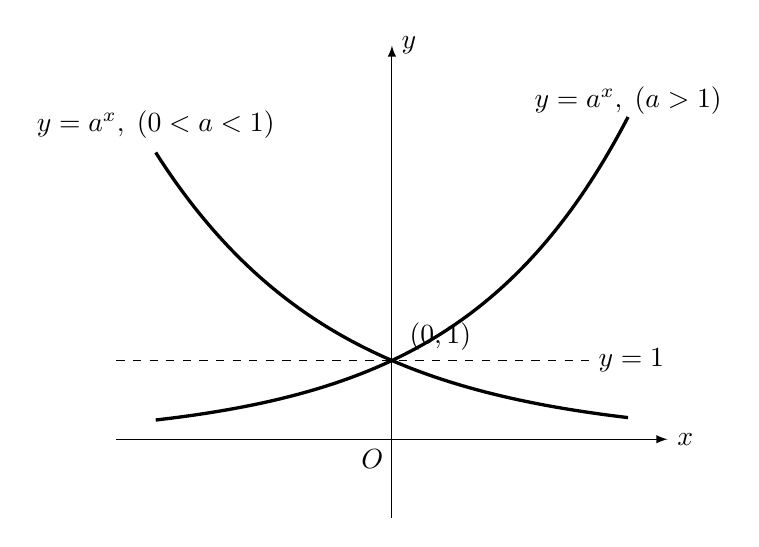
\begin{tikzpicture}[>=latex]
\draw[->](-3.5,0)--(3.5,0)node[right]{$x$};
\draw[->](0,-1)--(0,5)node[right]{$y$};
\draw[dashed] (-3.5,1)--(2.5,1)node[right]{$y=1$};
\draw [domain=-3:3, samples=100, very thick]plot(\x, {1.6^(\x)});
\draw [domain=-3:3, samples=100, very thick]plot(\x, {0.65^(\x)});
\node at (-3,4){$y=a^x,\; (0<a<1)$};
\node at (3,4.3){$y=a^x,\; (a>1)$};
\node at (-.25,-.25){$O$};
\node at (.1,1.3)[right]{$(0,1)$};
\end{tikzpicture}
  \caption{}\label{fig:4-10-3}
\end{figure}

\begin{Theorem}{逆定理}
  任何一个满足上述性质 1 和 2 的函数 $f(x)$ 必定是一个指数函数,其底为 $a=f(1)$。
\end{Theorem}
 
\begin{proof}
由性质 1, 对于任何实数 $x$,有
\[f(0)f(x)=f(0+x)=f(x)\]
即得,$f(0)=1$。 当 $f(x)$ 递增时,$f(1)=a>f(0)=1$,而当 $f(x)$ 递减时,$f(1)=a<f(0)=1$。

由性质 1:
\[\begin{split}
  f(m)&=f\big((m-1)+1\big)=f(m-1)\cdot f(1)\\
  &=f(m-2)\cdot \big(f(1)\big)^2=f(m-3)\cdot \big(f(1)\big)^3\\
  & \cdots  \\
  & =\big(f(1)\big)^m=a^m
\end{split}\]
又因为
\[\begin{split}
  \left[f\left(\frac{m}{n}\right)\right]^n&=f\overbrace{\left(\frac{m}{n}+\frac{m}{n}+\cdots +\frac{m}{n}\right)}^{n\text{个}}\\
  &=f(m)=a^m
\end{split}\]
所以:$f\left(\dfrac{m}{n}\right)=\sqrt[n]{a^m}=a^{\tfrac{m}{n}}$

因为 $f\left(\dfrac{m}{n}\right)f\left(-\dfrac{m}{n}\right)=f\left(\dfrac{m}{n}-\dfrac{m}{n}\right)=f(0)=1$

所以$f\left(-\dfrac{m}{n}\right)=\dfrac{1}{f\left(\dfrac{m}{n}\right)}=\dfrac{1}{a^{\tfrac{m}{n}}}=a^{-\tfrac{m}{n}}$

所以,$f(r)=a'$,对于正、负分数$r$都成立。

再由单调性,和实指数幂的定义,就可以说明 $f(x)=a^x$ 对于任何实数都成立。

设 $x\in\mathbb{R}$ 为一任意实数,$r_n\to x\leftarrow s_n$ 是 $x$ 的左、右夹逼有理数列,即
\begin{equation}
  \label{eq:pinch_sequence}
  r_1\leqslant r_2\leqslant\cdots \leqslant r_n\leqslant\cdots \leqslant x\leqslant\cdots \leqslant s_n\leqslant\cdots \leqslant s_2\leqslant s_1
\end{equation}
并且 $\lim(s_n-r_n)=0$。

由不等式 \eqref{eq:pinch_sequence} 和 $f(x)$ 的递增性(递减性),得到
\begin{equation}
  \label{eq:pinch_function}
  f(r_1)\leqslant f(r_2)\leqslant\cdots \leqslant f(r_n)\leqslant\cdots \leqslant f(x)\leqslant\cdots \leqslant f(s_n)\leqslant\cdots \leqslant f(s_2)\leqslant f(s_1)
\end{equation}
$r_n,s_n$ 都是有理数。
(若 $f(x)$ 递减,我们得到不等式 \eqref{eq:pinch_function} 的反向不等式)。

不等式 \eqref{eq:pinch_function} 可改写成
\begin{equation}
  \label{eq:pinch_function2}
  a^{r_1}\leqslant a^{r_2}\leqslant\cdots \leqslant a^{r_n}\leqslant\cdots \leqslant a^{x}\leqslant\cdots \leqslant a^{s_n}\leqslant\cdots \leqslant a^{s_2}\leqslant a^{s_1}
\end{equation}
而上节实数指数定义中,$a^x$ 是唯一能满足 \eqref{eq:pinch_function2} 的实数,所以 $f(x)=a^x$。

在上面的讨论中,$x$ 是一个任意的实数,因此,$f(x)=a^x$,对于任何实数 $x$ 恒成立。
\end{proof}

\begin{example}\label{eq:exponential_inequality}
设 $a,b$ 是不等的正实数,试证
\[a^ab^b>(ab)^{\tfrac{a+b}{2}}>a^bb^a\]
\end{example}

\begin{proof}
不妨设 $a>b$,则 $\dfrac{a}{b}>1$,$a-b>0$。于是,根据实指数幂性质 1,可得:
\[\frac{a^ab^b}{(ab)^{\tfrac{a+b}{2}}}=a^{\tfrac{a-b}{2}}\cdot b^{\tfrac{b-a}{2}}=\left(\frac{a}{b}\right)^{\tfrac{a-b}{2}}>1\]

由于 $a>0,\;  b>0\Rightarrow ab>0$,因此,$(ab)^{\tfrac{a+b}{2}}>0$,所以,有
\[a^ab^b>(ab)^{\tfrac{a+b}{2}}\]
另外,根据同样的道理,有
\[\frac{(ab)^{\tfrac{a+b}{2}}}{a^bb^a}=a^{\tfrac{a-b}{2}}\cdot b^{\tfrac{b-a}{2}}=\left(\frac{a}{b}\right)^{\tfrac{a-b}{2}}>1\]
又 $a^b>0$,$b^a>0$。 所以 $(ab)^{\tfrac{a+b}{2}}>a^b b^a$,这就证明了
\[a^ab^b>(ab)^{\tfrac{a+b}{2}}>a^b b^a\]
\end{proof}

\begin{Exercise}
\begin{question}
  \item 利用实指数幂的性质,指出下列不等式中,$a$ 是大于 1, 还是大于 0 而小于 1?
  \begin{tasks}(2)
    \task $a^{\sqrt{2}}<a^{\tfrac{\sqrt{2}}{2}}$
    \task $a^{-\sqrt{3}}>a^2$
    \task $a^{-\sqrt{5}-\sqrt{7}}>a^{-5}$
    \task $a^{1+\sqrt{5}}<a^{2+\sqrt{2}}$
    \task $a^{\sqrt{7}+\sqrt{2}}<a^{\sqrt{6}+\sqrt{3}}$
  \end{tasks}
  \item 作下列各函数的图象:
  \begin{tasks}(2)
    \task $y=3^x$
    \task $y=3^{-x}$
  \end{tasks}
  \item 
  \begin{tasks}
    \task 证明 $f(x)=\dfrac{2^x+2^{-x}}{2}$ 是偶函数,并作出它的图象;
    \task 当 $x$ 为何值时,$f(x)$ 有最小值,并求最小值。
  \end{tasks}
  \item 设 $a,b,c$ 是不等的正数,证明:
  \begin{tasks}
    \task $a^{2 a} b^{2 b} c^{2 c}>a^{b+c} b^{c+a} c^{a+b}$
    \task $a^{a} b^{b} c^{c}>(a b c)^{\tfrac{a+b+c}{3}}$
  \end{tasks}
  (提示:利用\cref{eq:exponential_inequality} 的结果)
  \item 证明:
  \begin{tasks}
    \task 当 $n$ 是 1 或不小于 5 的自然数时,总有 $2^n>n^2$;
    \task $\lim\limits_{n\to\infty}\dfrac{2^n}{n}=\infty$。
  \end{tasks}
\end{question}
\end{Exercise}

\section{对数函数}

由实数幂的定义,我们得知指数函数
\[a^x,\quad (a>0,\;a\ne 1),\qquad x\in\mathbb{R}\]
的值都是正的,现在还要进一步说明指数函数的值域是正实数集,也就是必须证明下面的命题。

\begin{Theorem}{命题}
给定不等于 1 的正实数 $a$,对于任意正数 $b$,一定存在唯一的一个实数 $c$,满足下列方程
\[a^c=b\]
\end{Theorem}

\begin{proof}
为确定起见,设 $a>1$,依实指数函数的性质 5,$\lim\limits_{x\to-\infty}a^x=0$,可以找出这样一数 $c_1$ 以使 $a^{c_1}<b$,依 $a^x,\;(a>1)$ 是增函数且$\lim\limits_{x\to+\infty}a^x=+\infty$,可以找出这样的数 $c_2>c_1$,以使 $a^{c_2}>b$,现在由连续函数中间值定理知道,在 $c_1$ 与 $c_2$ 之间有实数 $c$ 以使 $a^c=b$,再由单调性知道这个数是唯一的。类似地可以证明 $0<a<1$ 的场合,这个证明留给同学补全。
\end{proof}


现在我们根据第八章第五节反函数定理可以说由指数函数得到一个定义在正实数变域上的反函数,称为对数函数,记作 $f:\mathbb{R}^+\mapsto \mathbb{R}$,这里 $f(x)=\log_a x$,它是连续的单调函数。正式定义如下:

\begin{Definition}
若 $a>0$ 且 $a\ne 1$,那么 $y=\log_a x$,当且仅当 $x=a^y$。我们称 $y$ 是以 $a$ 为底的对数,函数 $f:\mathbb{R}^+\mapsto \mathbb{R}$,这里 $f(x)=\log_a x$ 称为\Concept{对数函数}。
\end{Definition}

这个定义导致下面有用的结果:
\begin{enumerate}[itemsep=5pt]
  \item $a^{\log_a x}=x,\qquad \log_a a^x=x$
  \item $\log_a (xy)=\log_a x+\log_a y$
  \item $\log_a \dfrac{x}{y}=\log_a x-\log_a y$
  \item $\log_a x^r=r\log_a x$
  \item $\log_a b=\dfrac{\log_c b}{\log_c a}$(换底公式)。
\end{enumerate}
证明过程请看第三册第一章。

从函数的图象来说:$y=\log_a x,\; (x\in\mathbb{R})$ 的图象能由 $y=a^x,\; (x\in\mathbb{R})$ 的图象经 $y=x$ 的反射而得到,如\cref{fig:4-10-4}。
\begin{figure}
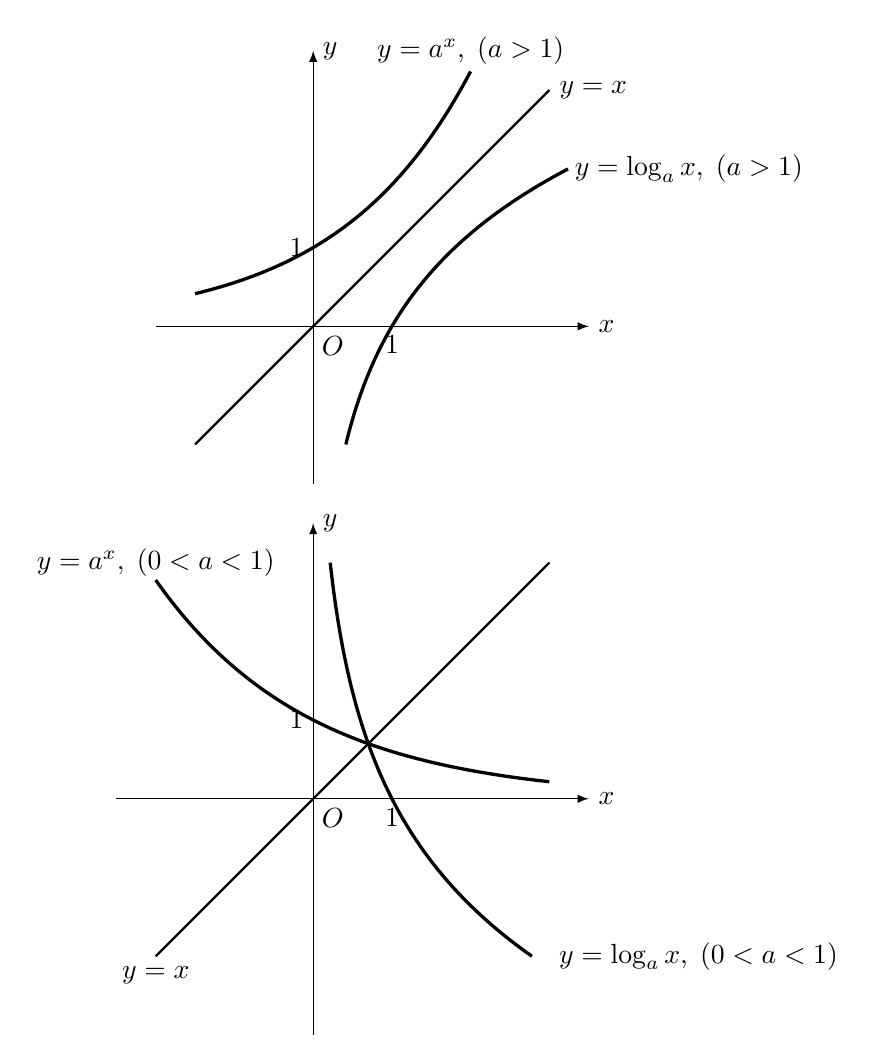
\begin{tikzpicture}[>=latex]
\begin{scope}
  \draw[->](-2,0)--(3.5,0)node[right]{$x$};
\draw[->](0,-2)--(0,3.5)node[right]{$y$};
\draw[thick] (-1.5,-1.5)--(3,3)node[right]{$y=x$};
\draw[domain=-1.5:2, samples=100, very thick]plot(\x,{1.8^(\x)});
\draw[domain=-1.5:2, samples=100, very thick]plot({1.8^(\x)},\x);
\node at (2,3.5){$y=a^x,\; (a>1)$};
\node at (3.2,2)[right]{$y=\log_a x,\; (a>1)$};
\node at (1,0)[below]{1};
\node at (0,1)[left]{1};
\node at (.25,-.25){$O$};
\end{scope}
\begin{scope}[yshift=-6cm]
  \draw[->](-2.5,0)--(3.5,0)node[right]{$x$};
  \draw[->](0,-3)--(0,3.5)node[right]{$y$};
  \draw[thick] (-2,-2)node[below]{$y=x$}--(3,3);
  \draw[domain=-2:3, samples=100, very thick]plot(\x,{0.6^(\x)});
  \draw[domain=-2:3, samples=100, very thick]plot({0.6^(\x)},\x);
  \node at (-2,3){$y=a^x,\; (0<a<1)$};
\node at (3,-2)[right]{$y=\log_a x,\; (0<a<1)$};
\node at (1,0)[below]{1};
\node at (0,1)[left]{1};
\node at (.25,-.25){$O$};
\end{scope}
\end{tikzpicture}
  \caption{}\label{fig:4-10-4}
\end{figure}

由于 $x$ 轴是指数函数图象的渐近线,故 $y$ 轴是对数函数图象的渐近线。相应于指数函数的极限值:
\[\begin{split}
  \lim_{x\to -\infty} a^x=0&,\qquad a>1\\
  \lim_{x\to +\infty} a^x=0&,\qquad 0<a<1
\end{split}\]
有对数函数的极限值:
\[\lim_{x\to 0^+} \log_a x=\begin{cases}
  -\infty, & a>1\\
  +\infty ,& 0<a<1
\end{cases}\]

相应于指数函数的特征性质,也就有对数函数的特征性质:
\begin{enumerate}
  \item $\log_a (x_1\cdot x_2)=\log_a x_1+\log_a x_2$
  \item 单调性。当 $a>1$ 递增;当 $0<a<1$ 递减。
  \item 连续性。即在 $(0,+\infty)$ 内处处连续。同样地,对应于第三节中的定理,总结成下面的定理。
\end{enumerate}

\begin{Theorem}{定理}
对数函数 $f(x)=\log_a x$ 满足下列性质:
  \begin{enumerate}
    \item $f(x_1\cdot x_2)=f(x_1)+f(x_2)$
    \item 单调性。$a>1$ 时,递增;$0<a<1$ 时,递减。
    \item 在 $x>0$ 半直线上,处处连续。
  \end{enumerate}
\end{Theorem}
 
\begin{Theorem}{逆定理} 
  任何一个满足性质 1、2 的函数 $f(x) $一定是一个对数函数,即存在适当的 $a$,使得 $f(x)=\log_a x$。
\end{Theorem}

\begin{proof}
由性质 1,$f(x_1)=f(x_1\cdot 1)=f(x_1)+f(1)$。因此 $f(1)=f(x_1)-f(x_2)=0$。

我们先任取一常数 $A>1$,则由性质 2 知
\[f(A)\ne f(1)=0\]
再由性质 1
\[f(A^m)=\underbrace{f(A)+f(A)+\cdots+f(A)}_{\text{$m$项}}=mf(A),\qquad m\in\mathbb{N}\]

又
\[\begin{split}
  mf(A)&=f(A^m)=f\left(\left((A)^{\tfrac{m}{n}}\right)^n\right)\\
  &=\underbrace{f\left(A^{\tfrac{m}{n}}\right)+\cdots+f\left(A^{\tfrac{m}{n}}\right)}_{\text{$n$项}}=nf\left(A^{\tfrac{m}{n}}\right)
\end{split} \]
$\therefore\quad f\left(A^{\tfrac{m}{n}}\right)=\frac{m}{n}f(A),\qquad m,n\in\mathbb{N}$

又$\because\quad f\left(A^{\tfrac{m}{n}}\right)+f\left(A^{-\tfrac{m}{n}}\right)=f\left(A^{\tfrac{m}{n}}\cdot A^{-\tfrac{m}{n}}\right)=f(A^0)=f(1)=0$

$\therefore\quad f\left(-A^{\tfrac{m}{n}}\right)=-f\left(A^{\tfrac{m}{n}}\right)=-\frac{m}{n}f(A)$

\bigskip
综合上面所证,所以对于所有有理数 $r\in\mathbb{Q}$,都有
\[f(A^r)=rf(A)\]
从此不难用单调性和极限过程,导出
\begin{equation}
  \label{eq:logarithmic_function}
  f(A^{\beta })=\beta f(A),\qquad \beta \in\mathbb{R}
\end{equation}

令 $A^{\beta }=x$,则 $\beta =\log_A x$,于是\cref{eq:logarithmic_function} 可写成
\begin{equation}
  \label{eq:logarithmic_function2}
  f(x)=f(A)\cdot \log_A x
\end{equation}
这样我们得到一个连续的单调的对数型函数\cref{eq:logarithmic_function2}。为了化去常数因子 $f(A)$,我们要用一些技巧如下:令 $a=A^{\tfrac{1}{f(A)}}$,于是
\[1=\log_a a=\log_a A^{\tfrac{1}{f(A)}}=\frac{1}{f(A)}\cdot \log_a A\]
即:$f(A)=\log_a A$,代入\cref{eq:logarithmic_function2},得到:
\[f(x)=\log_A x\cdot \log_a A=\log_a x\]
\end{proof}

\begin{Exercise}
\begin{question}
  \item 求下列各函数的定义域与值域,如果它们是可逆的,写出以 $x$ 为自变数的反函数。
  \begin{tasks}(2)
    \task $y=\log_2(x-2)$
    \task $y=\log_2\dfrac{1}{x}$
    \task $y=e^{-x}$
    \task $y=\sqrt{\lg\cos2\uppi x}$
  \end{tasks}
  \item 计算下列各式的值:
  \begin{tasks}(2)
    \task $2^{\log_4 9}$
    \task $5^{\log_{0.2} 7}$
    \task $3^{\log_{\sqrt{2}}6}$
    \task $6^{1+\log_6 5}$
    \task $25^{\tfrac{1}{3} \log 5^{27}-\log_{5} 4}$
    \task $10^{\lg\sqrt{100}}$
    \task $\log _{\sqrt{4-\sqrt{15}}} \sqrt{4+\sqrt{15}}$
    \task $4-\lg 8-3 \lg 5$
    \task $ \lg ^{2} 5+\lg 2 \lg 50$
    \task $\dfrac{3 \lg 1728}{1+\dfrac{1}{2} \lg 0.36+\dfrac{1}{3} \lg 8}$
    \task $\log _{a} b \cdot \log _{b} c \cdot \log _{c} d$
    \task $\left(\log _{2} 3+\log _{4} 9\right)\left(\log _{3} 4+\log _{9} 2\right)$
  \end{tasks}
  \item 证明下面的恒等式:
  \begin{tasks}(2)
    \task $\log_a b=\dfrac{\log_c b}{\log_c a}$
    \task $\log_a b\cdot \log_b a=1$
    \task! $\dfrac{\log_a x}{\log_{ab} x}=1+\log_a b$  
    \task! \[\begin{split}
      &\quad \frac{1}{(\log_x 2)(\log_x 4)}+   \frac{1}{(\log_x 4)(\log_x 8)}+   \frac{1}{(\log_x 8)(\log_x 16)}+\cdots \\
      &+   \frac{1}{(\log_x 2^{n-1})(\log_x 2^n)}=\left(1-\frac{1}{n}\right)\left(\frac{1}{\log_x 2}\right)^2
    \end{split}\]
  \end{tasks}
  \item 
  \begin{tasks}
    \task 已知 $\lg2=a$,$\lg7=b$,求 $\log_8 9.8$;
    \task 已知 $\log_{18}9=a$,$\log_{18}5=b$,求 $\log_{36}45$;
    \task 已知 $\lg198=2.2966$,$\lg2=0.3010$,$\lg3=0.4771$,求 $\lg 11$;
    \task 已知 $\log_{12}7=m$,$\log_{12}3=n$,求 $\log_{18}63$。
  \end{tasks} 
  \item 已知 $\lg3=0.4771$,问 $\left(\dfrac{1}{3}\right)^{20}$ 表成小数时,不等于 0 的第一个有效数字出现在哪里?
  \item 证明下面不等式:
  \begin{tasks}
    \task $\left|\log _{a} b\right|+\left|\log _{b} a\right| \geqslant 2$
    \task $\dfrac{1}{\log _{2} \uppi}+\dfrac{1}{\log _{\uppi} 2}>2$
    \task 若 $a>b>0$ 且 $c>1$,则 $\log _{c} \dfrac{b}{a}<\log _{c} \dfrac{1+b}{1+a}$。
    \task 若 $t>-1$,$\varphi(t)=-\lg(1+t)$,则 $\varphi\left(\dfrac{t_{1}+t_{2}}{3}\right)<\dfrac{\varphi\left(t_{1}\right)+\varphi\left(t_{2}\right)}{2}$
  \end{tasks}
  \item 当 $2 x+5 y=20$ 时, 求 $\log _{2} x+\log _{2} y$ 的最大值。
  \item 设 $x>1$,$y>1$ 且 $2 \log _{x} y-2 \log _{y} x+3=0$,那么 $x^{2}-$ $4 y^{2}$ 的最小值是多少?
  \item 设 $x>2$,$y>2$,比较下列各式的大小:
  \[\log _{2} \frac{x+y}{2} ;\qquad \frac{1}{2} \log _{2}(x+y); \qquad \frac{1}{2}\left(\log _{2} x+\log _{2} y\right)\]
  \item  求证等比数列的各项的对数组成等差数列。
  \item  有等比数列, 它的公比为 2, 项数为10, 如果各项 取以2 为底的对数, 它们的和是 25, 求这等比数列的和。
  \item 试问数列
  $$\lg100,\; \lg\left(100\sin\frac{\uppi}{4}\right),\; \lg\left(100\sin^2\frac{\uppi}{4}\right),\; \ldots ,\; \lg\left(100\sin^{n-1}\frac{\uppi}{4}\right),\; \ldots$$
  的前多少项的和的值最大?并求出最大值(这里取 $\lg2=0.3010$)。
\end{question}
\end{Exercise}

\section{指数方程与对数方程}
指数中含有未知数的方程叫做\Concept{指数方程}。下面我们介绍几种常见的指数方程及其解法。

\subsection{可化为 \texorpdfstring{$\alpha^{f(x)}=\alpha^{g(x)}\; (a>0\text{\;且\;}a\neq 1)$}{} 的指数方程}
对于这类方程,我们根据指数函数的单调性得到 $\alpha^{f(x)}=\alpha^{g(x)}$ 成立的必要充分条件是 $f(x)=g(x)$。 因此,指数方程 $\alpha^{f(x)}=\alpha^{g(x)}$ 在 $a>0$ 且 $a\ne 1$ 的条件下就可以转化为代数方程 $f(x)=g(x)$ 来解。

\begin{example}
  解方程 $5^{-x}\cdot 50^x=\dfrac{1}{1000(10^{2x-1})^{-3}}$
\end{example}

\begin{solution}
原方程化简为 $(5^{-1}\cdot 50)^x=\dfrac{10^{6x-3}}{10^3}$,即:
\[10^x=10^{6x-6}\]

由于底数 $a=10>0$ 且 $\ne 1$,得到
\[x=5x-6 \quad \Rightarrow\quad x=\frac{6}{5}\]
所以原方程的解集是 $\left\{\dfrac{6}{5}\right\}$。
\end{solution}


\begin{example}
解方程 $17^{3x^2+x-2}=1$
\end{example}

\begin{solution}
$\because\quad 1=17^0$,原方程可写成
\[17^{3x^2+x-2}=17^{0}\]
于是根据指数函数的单调性,得到
\[3x^2+x-2=0\]
由此
\[x_1=\frac{2}{3},\qquad x_2=-1\]
所以 原方程的解集是 $\left\{-1,\dfrac{2}{3}\right\}$。
\end{solution}

\subsection{可化为形如 $a^{f(x)}=b^{g(x)}$ 的指数方程}
这里($a>0$,$b>0$,$a\ne 1$,$b\ne 1$),一般用两边取对数的方法来解。

\begin{example}
解方程 $17^x=300$
\end{example}

\begin{solution}
两边取常用对数,得到
\[\begin{split}
  x\lg17&=\lg300\\
  x&=\frac{\lg300}{\lg 17}\approx \frac{2.4771}{1.2304}\approx 2.0132
\end{split}\]  
\end{solution}  
  
\begin{example}
  解方程 $5^{2x}-7x-35\cdot 5^{2x}+35\cdot 7^x=0$
\end{example}

\begin{solution}
原方程化简为 $7^x (35-1)=5^{2x}(35-1)$

两边除以 34, 得到:$5^{2x}=7^x$

两边取常用对数
\[\begin{split}
  2x\lg5&=x\lg7\\
x(2\lg5-\lg7)&=0
\end{split} \]
$\because\quad   2\lg5-\lg7=\lg25-\lg7\ne 0,\qquad \therefore\quad x=0$

因此,原方程的解集是 $\{0\}$。
\end{solution}

\subsection{可化为一元二次方程的指数方程}

\begin{example}
解方程 $\left(\sqrt{2-\sqrt{3}}\right)^x+\left(\sqrt{2+\sqrt{3}}\right)^x=4$
\end{example}

\begin{solution}
注意到 $\sqrt{2-\sqrt{3}}\cdot \sqrt{2+\sqrt{3}}=\sqrt{4-3}=1$,原方程的两边乘以 $\left(\sqrt{2-\sqrt{3}}\right)^x$,得到
\[\left(\sqrt{2-\sqrt{3}}\right)^{2x}+1=4\left(\sqrt{2-\sqrt{3}}\right)^x\]
即
$\left(\sqrt{2-\sqrt{3}}\right)^{2x}-4\left(\sqrt{2-\sqrt{3}}\right)^x+1=0$

$\therefore\quad \left(\sqrt{2-\sqrt{3}}\right)^x=2+\sqrt{3}\quad \text{或}\quad \left(\sqrt{2-\sqrt{3}}\right)^x=2-\sqrt{3}$

即:
\[\left({2-\sqrt{3}}\right)^{\tfrac{x}{2}}=\left({2-\sqrt{3}}\right)^{-1}\quad \text{或}\quad \left({2-\sqrt{3}}\right)^{\tfrac{x}{2}}=2-\sqrt{3}\]
$\therefore\quad x=-2\quad \text{或}\quad x=2$

$\therefore\quad $原方程的解集是$\{-2,2\}$。
\end{solution}

未知数前面有对数符号的方程称为对数方程。解对数方程一般常用的方法是根据对数定义直接把对数式的等式写成指数形式的等式。也有时根据对数函数的单调性把对数方程化为代数方程来解。但是必须注意在解对数方程之前,应该先确定使方程中的对数都有意义的定义域,由此便确定了方程的根的上、下界。在求得对数方程之解后,应该舍去在根的上、下界之外的增根,换言之,把那些使真数或底数为非正数或使底数等于1的根舍去,下面介绍几种常见的对数方程。

\subsection{形如 $\log_{f(x)}g(x)=c$\; (其中 $c$ 是常数)的对数方程}

可以根据对数定义将它化为指数形式的等式去解。
\begin{example}
解方程 $\log_{x-5}(3x^2-16x+29)=2$
\end{example}

\begin{solution}
方程中的对数有意义必须
\[\begin{cases}
  x>5\quad\text{且}\quad  x-5\ne 1 \\
  13x^2-16x+29>0
\end{cases}\] 
根据对数定义得到
\[ 3x^2-16x+29=(x-5)^2\]
解得:$x_1=1,\qquad x_2=2$。

由于 1 和 2 都小于 5, 所以原方程没有解,即原方程的解集是空集。
\end{solution}

\begin{example}
解方程 $\log_3[3+2\lg(1+x)]=0$
\end{example}

\begin{solution}
根据对数定义得到 $3+2\lg(1+x)=1$,即:
\[\lg(1+x)=-1\]
再由对数定义有
\[\begin{split}
  1+x&=10^{-1}\\
  x&=-0.9
\end{split}\]  
经验算可知原方程的解集是 $\{-0.9\}$。
\end{solution}

\subsection{可以化成形如 $\log_a f(x)=\log_a g(x)$ 的对数方程}

由对数函数的单调性知道,上面方程成立的充分必要条件是
\[\begin{cases}
  f(x)>0\\
  g(x)>0\\
  f(x)=g(x)
\end{cases}\]
因此对数方程可化为代数方程和不等式来解。

\begin{example}
解方程 $\lg x+\lg(x^2-4)=\lg3+\lg(x+2)$
\end{example}

\begin{solution}
方程中的对数有意义,必须
\[\begin{cases}
  x>0\\
  x^2-4>0\quad \Rightarrow\quad  x>2\\
  x+2>0
\end{cases}\]
原方程化为 $\lg x(x^2-4)=\lg 3(x+2)$,由此得到
\[x(x^2-4)=3(x+2)\]
即:$(x-2)(x^2-2x-3)=0$,
解得:
\[x_1=2,\qquad x_2=-1,\qquad x_3=3\]
其中只有 $x_3=3>2$,所以原方程的解集是 $\{3\}$。
\end{solution}

根据指数函数与对数函数的单调性也可以解相应的一些不等式。由于作对数变形时,也有可能把原来数的定义域缩小了,这时就会丢掉解,因此,作对数变形时,应该避免这种情形发生。例如,解 $\lg x^2=1$,如果利用等式:$\lg x^2=2\lg x$,把原方程变形为 $2\lg x=1$,这时由这个方程只能解出 $x=\sqrt{10}$,丢失了原方程的一个根 $-\sqrt{10}$。

\begin{example}
  解不等式 $\log_{\tfrac{1}{3}}[\log_4 (x^2-5)]>0$
\end{example}

\begin{solution}
  原不等式等价于 $0<\log_4(x^2-5)<1$,由此 $1<x^2-5<4$,即:
\[6<x^2<9\]
$\therefore\quad \sqrt{6}<|x|<3$
从而:
\[\sqrt{6}<x<3\quad \text{或}\quad -3<x<-\sqrt{6}\]
\end{solution}

\begin{example}
  解 $\log_a x>6\log_x a-1,\qquad (0<a<1)$
\end{example}

\begin{solution}
  原不等式可写成
\begin{equation}
  \label{eq:inequality1}
  \log_a x>\frac{6}{\log_a x}-1
\end{equation}
分两种情形来解:
\begin{enumerate}
  \item 设 $0<x<1$,则 $\log_a x>0,\quad (0<a<1)$。
  
由\cref{eq:inequality1} 得 $\log_a^2 x+\log_a x-6>0$,由此得:
\begin{equation}
  \label{eq:solution1}
  \log_a x<-3
\end{equation}
或
\begin{equation}
  \label{eq:solution2}
  \log_a x>2
\end{equation}
由\cref{eq:solution1} 得 $x>\dfrac{1}{a^3}>1$,这与前设 $0<x<1$ 矛盾。所以\cref{eq:solution1} 无解。

由\cref{eq:solution2} 得 $0<x<a^2<1$,因此由\cref{eq:inequality1} 得:$0<x<a^2$

\item 设 $x>1$,则 $\log_a x<0,\quad (0<a<1)$。

由\cref{eq:inequality1} 得 $\log_a^2 x+\log_a x-6<0$,由此得:
\[-3<\log_a x<2\]
$\because\quad 0<a<1,\qquad \therefore\quad a^2<1<x<a^{-3}$

因此,由\cref{eq:inequality1} 可得,$1<x<\dfrac{1}{a^3}$。

$\therefore\quad $ 原不等式的解集是 $\left\{x|0<x<a^2\right\}\cup\left\{x\Big|1<x<\dfrac{1}{a^3}\right\}$
\end{enumerate}
\end{solution}

\begin{example}
  解不等式 $\dfrac{1}{\log_2 x}-\dfrac{1}{\log_2 x-1}<1$
\end{example}

\begin{solution}
  原不等式可化简为 $\dfrac{1+\log_2 x(\log_2 x-1)}{\log_2 x(\log_2 x-1)}>0$,即:
\[\frac{\left(\log_2 x-\frac{1}{2}\right)^2+\dfrac{3}{4}}{\log_2 x(\log_2 x-1)}>0\]
由此得:$\log_2 x(\log_2 x-1)>0$,因此:
\[\log_2 x<0\quad \text{或}\quad \log_2 x>1\]
即:$0<x<1\quad \text{或}\quad x>2$。

由此原不等式的解集是 $\{x|0<x<1\}\cup\{x|x>2\}$。
\end{solution}

\begin{example}
  求函数 $f(x)=\sqrt{\log_{\tfrac{1}{2}}\dfrac{x}{x^2-1}}$ 的定义域。
\end{example}

\begin{solution}
\[\begin{split}
  \text{函数$f$有意义}&\Longleftrightarrow \log_{\tfrac{1}{2}}\frac{x}{x^2-1}\text{有意义}\Longleftrightarrow \log_{\tfrac{1}{2}}\frac{x}{x^2-1}\geqslant 0\\
  &\Longleftrightarrow  0<   \frac{x}{x^2-1}\leqslant1    \Longleftrightarrow  \begin{cases}
    \dfrac{x}{x^2-1}>0\\ \dfrac{x^2-x-1}{x^2-1}\geqslant 0
  \end{cases}           \\
  &\Longleftrightarrow     \begin{cases}
    -1<x<0\quad \text{或}\quad x>1\\
    x<-1\quad \text{或}\quad \dfrac{1-\sqrt{5}}{2}<x<1\quad \text{或}\quad x>\dfrac{1+\sqrt{5}}{2}
  \end{cases}               \\
  &\Longleftrightarrow   \begin{cases}
    -1<x<0\\  \dfrac{1-\sqrt{5}}{2}<x<1
  \end{cases}      \text{或}\quad  \begin{cases}
    x>1\\x>\dfrac{1+\sqrt{5}}{2}
  \end{cases}           \\
  &\Longleftrightarrow    \dfrac{1-\sqrt{5}}{2}<x<1  \quad \text{或}\quad   x>\frac{1+\sqrt{5}}{2}   \\
\end{split}\]
故函数 $f$ 的定义域为
\[\left\{x\Big| \frac{1-\sqrt{5}}{2}<x<1 \right\}\bigcup\left\{x\Big|x>\frac{1+\sqrt{5}}{2}  \right\}\]
\end{solution}


\begin{example}
  解方程 $\log_{\sin 3x}(\cos x-\cos2x)=1$
\end{example}

\begin{solution}
  要使方程中的对数有意义,$x$ 必须满足条件:
\begin{equation}
  \begin{cases}
    \sin 3x>0\quad \text{且}\quad \sin3 x\ne 1\\
    \cos x-\cos2x>0
  \end{cases}
\end{equation}
由原方程得 $\cos x-\cos2x=\sin3x$,即:
\[\sin \frac{3x}{2}\left(\sin \frac{x}{2}-\cos\frac{3x}{2}\right)=0\]
由此得:
\[\sin\frac{3x}{2}=0\quad \text{或}\quad \sin \frac{x}{2}-\cos\frac{3x}{2}=0\]
因为 $\sin\dfrac{3x}{2}=0$的解,根据$\sin3x=2\sin\dfrac{3x}{2}\cos\dfrac{3x}{2}$,知道一定也使 $\sin 3x=0$ 成立,而这与 $x$ 满足的条件:$\sin3x>0$
不合,因此,方程 $\sin\dfrac{3x}{2}=0$ 的解应该舍去。

由$\sin \dfrac{x}{2}-\cos \dfrac{3x}{2}=0$,得:
\[\sin \frac{x}{2}=\sin \left(\frac{\uppi}{2}-\frac{3x}{2}\right)\]
根据两角正弦相等条件,有
\[\frac{x}{2}=\frac{\uppi}{2}-\frac{3x}{2}+2k\uppi\quad \text{或}\quad \frac{x}{2}=\frac{\uppi}{2}+\frac{3x}{2}+2k\uppi\]
即:
\begin{equation}
x=\frac{\uppi}{4}+k\uppi
\end{equation}
或
\begin{equation}
  x=-\frac{\uppi}{2}-2k\uppi
\end{equation}
在单位圆上,分别作出(10.11)中和(10.12)中的诸角的终边,如\cref{fig:4-10-5}。

\begin{figure}[htp]
  \centering
\begin{tikzpicture}[>=latex]
\begin{scope}
  \draw[->] (-2,0)--(2,0)node[right]{$x$};
  \draw[->] (0,-1.5)--(0,2)node[right]{$y$};
\draw[thick] (0,0) circle (1);
\draw[very thick,->] (1,0) arc (0:180+45:1);
\draw[thick, <->] (45:1)node[above]{$\dfrac{\uppi}{4}$}--(180+45:1)node[below]{$\dfrac{5\uppi}{4}$};
\node at (.25,-.25){$O$};
\node at (1.4,0)[below]{$(1,0)$};
\node at (0,-2.2){$x=\dfrac{\uppi}{4}+2k\uppi$};
\end{scope}
\begin{scope}[xshift=5cm]
  \draw[->] (-2,0)--(2,0)node[right]{$x$};
  \draw[->] (0,-1.5)--(0,2)node[right]{$y$};
  \draw[thick] (0,0) circle (1);
\draw[very thick,->] (1,0) arc (0:-90:1);
\draw[thick, ->] (0,0)--(-90:1);
\node at (-.25,-.25){$O$};\node at (1.4,0)[below]{$(1,0)$};
\node at (0,-2.2){$x=-\dfrac{\uppi}{2}+2k\uppi$};
\end{scope}
\end{tikzpicture}
  \caption{}\label{fig:4-10-5}
\end{figure}

显然(10.11)又可写成
\begin{equation}
  x=\frac{\uppi}{4}+2k\uppi
\end{equation}
和
\begin{equation}
  x=\frac{5\uppi}{4}+2k\uppi
\end{equation}
再由(10.12), (10.13), (10.14)容易看出角 $3x$ 与角 $-\dfrac{3\uppi}{2}$,$\dfrac{3\uppi}{4}$ 和 $-\dfrac{\uppi}{4}$ 有相同的终边,所以若将式(10.12)和式(10.14)代入 $\sin3x$ 中,便得到
\[\begin{split}
  \sin 3\left(-\frac{\uppi}{2}-2k\uppi\right)&=\sin\left(-\frac{3\uppi}{2}\right)=-\sin\frac{3\uppi}{2}=1\\
  \sin 3\left(\frac{5\uppi}{4}+2k\uppi\right)&=\sin\frac{15\uppi}{4}=\sin\left(4\uppi-\frac{\uppi}{4}\right)=\sin\left(-\frac{\uppi}{4}\right)=-\frac{\sqrt{2}}{2}<0
\end{split}\]
因此这两组解是增解,应该舍去,经检验知 $x=\frac{\uppi}{4}+2k\uppi$ 满足不等式组, 所以方程的解集是 $\left\{x\Big|x=\dfrac{\uppi}{4}+2k\uppi,\quad k\in\mathbb{Z}\right\}$。

\end{solution}

\begin{Exercise}
\begin{question}
  \item 解下列各指数方程:
  \begin{tasks}(2)
    \task $\displaystyle 3^{2 x-1}=81$
    \task $\displaystyle \sqrt{5^{x}}=\sqrt[3]{25}$
    \task $\displaystyle \sqrt[4]{7^{x}}=\sqrt[5]{343}$
    \task $\displaystyle \sqrt[4]{a^{x+1}}=\sqrt[3]{a^{x-3}}$ $(a>0,\;  a \neq 1)$
    \task $\displaystyle \sqrt{2^{x}} \sqrt{3^{x}}=36$
    \task $\displaystyle \left(\frac{3}{4}\right)^x=\left(\frac{4}{3}\right)^5$
    \task $\displaystyle \left(\frac{4}{9}\right)^{4}=\left(\frac{3}{2}\right)^{x}$
    \task $\displaystyle \left(\frac{2}{3}\right)^{x}\left(\frac{9}{8}\right)=\frac{27}{64}$
    \task $\displaystyle  4^{\sqrt{x+1}}=64 \cdot 2^{\sqrt{x+1}} $
    \task $\displaystyle (0.25)^{x-2}=\frac{256}{2^{x+3}}$
    \task $\displaystyle \left(\frac{4}{9}\right)^{x}\left(\frac{27}{8}\right)^{x-1}=\frac{2}{3}$
    \task $\displaystyle 2^{x} \cdot 5^{4}=0.1\left(10^{x-1}\right)^{5}$
  \end{tasks}
  \item  解下列各指数方程:
  \begin{tasks}(2)
    \task  $3^{x+2}+3^{x-1}=28$
    \task  $5^{x+1}-5^{x-1}=24$
    \task  $3^{2 x-1}+3^{2 x-2}-3^{2 x-4}=315$
    \task  $3^{x}+3^{x+1}+3^{x+2}=5^{x+1}+5^{x+2}$
    \task  $4^{x}+2^{x+1}=80$ 
    \task  $ 3^{x+2}+9^{x+1}-810=0$
    \task  $3^{2 x+5}=3^{x+2}+2$
    \task  $3^{4 \sqrt{x}}-4.3^{2 \sqrt{x}}+3=0$
    \task  $4.9^{\sqrt{x}-2}-3.15^{\sqrt{x}-2}=25^{\sqrt{x}-2} $
    \task  $4^{2 x}-2.18^{2 x}=3.81^{28} $
    \task! $\left(\sqrt{5+2 \sqrt{6}}\right)^{x}+\left(\sqrt{5-2 \sqrt{6}}\right)^{x}=\dfrac{10}{3}$
  \end{tasks}
  \item  求最小整数指数 $x$,使
  \begin{tasks}(2)
    \task $\displaystyle \left(\frac{4}{5}\right)^{x}<0.000001$
    \task $\displaystyle \left(\frac{3}{5}\right)^{x}<0.0001$
    \task $\displaystyle \left(\frac{10}{9}\right)^{x}>1000000$
    \task $\displaystyle \left(\frac{4}{5}\right)^{x}>10000000$
  \end{tasks}
  \item  解下列各不等式
  \begin{tasks}(2)
    \task  $\displaystyle 3^{3-5 x}-\frac{1}{81}>0$
    \task  $\displaystyle (0.3)^{2 x^{2}+5 x+2}<1$
    \task  $\displaystyle 8^{x}+16^{\tfrac{3}{4} x+1}<34$
    \task  $\displaystyle \frac{(0.5)^{3 x^{2}+10 x+6}}{100}<0.00125$
    \task  $\displaystyle 2^{x+1} \cdot 5^{2 x-3}<\frac{24}{25}$
    \task  $\displaystyle 5^{2x}-30.5^{x}+125<0$
    \task  $\displaystyle 2^{3 x}-2^{x+1}<2^{3} $
    \task  $\displaystyle \frac{1}{\left(\dfrac{1}{10}\right)^{y}-1} \leqslant \frac{2}{\left(\dfrac{1}{100}\right)^{y}-10}$
    \task  $\displaystyle \frac{1}{2^{x}-1} \geqslant \frac{1}{4^{x}-3}$
    \task  $\displaystyle \left(\frac{3}{4}\right)^{x-2}\left(\frac{4}{3}\right)^{\tfrac{1}{x}}>\frac{9}{16}$
  \end{tasks}
  \item  解下列各对数方程:
  \begin{tasks}(2)
    \task  $\lg x=2-\lg 5$
    \task  $\dfrac{2\lg x}{\lg(5x-4)}=1$
    \task  $\dfrac{\lg x}{1-\lg x}=2$
    \task  $\log_{x-1}(x^2-5x+10)=2$
    \task  $2 \lg x=-\lg \left(6-x^{2}\right)$
    \task  $\dfrac{1}{5-\lg x}+\dfrac{1}{1+\lg x}=1$
    \task  $0.5 \lg (2 x-1)+\lg \sqrt{x-9}=1$
    \task  $\log _{2} \log _{3} \log _{4} x=0$
    \task  $\lg 9^{-1}+x \lg \sqrt[3]{3^{5 x-7}}=0$
    \task  $\lg 10^{\lg\left(x^{2}+21\right)}-1=\lg x$
    \task! $\lg(x+6)-\dfrac{1}{2}\lg(2x-3)=2-\lg 25$
  \end{tasks}
  \item 解下列各对数方程:
  \begin{tasks}(2)
    \task   $\displaystyle 2 \log _{4} x+2 \log _{x} 4=5$ 
    \task   $\displaystyle \log _{2}(x-1)^{2}-\log _{0.5}(x-1)=9$
    \task   $\displaystyle \log _{8} x+\log _{4} x+\log _{2} x=7$
    \task   $\displaystyle \log _{x}\left(5 x^{2}\right) \cdot\left(\log _{5} x\right)^{2}=1$
    \task   $\displaystyle \sqrt{\log _{x} \sqrt{3 x}} \cdot \log _{3} x=-1$
    \task   $\displaystyle \log _{3 x}\left(\frac{3}{x}\right)+\log _{3}^{2} x=1$
    \task   $\displaystyle \frac{\lg\left(\sqrt{x+1}+1\right)}{\lg\sqrt[3]{x-40}}=3$
    \task!  $\displaystyle \sqrt{\log _{x} 5 \sqrt{5}+\log _{\sqrt{5}} 5 \sqrt{5}} \cdot \log _{\sqrt{5}} x=-\sqrt{6}$
  \end{tasks}
  \item 解下列各方程:
  \begin{tasks}(2)
    \task $(0.4)^{\lg^2 x+1}=(6.25)^{2-\lg x^3}$
    \task $x^{\lg x+2}=1000$
    \task $\sqrt{x^{\lg \sqrt{x}}}=10$
    \task $\lg x+\lg \sqrt[3]{x}+\lg  \sqrt[9]{x}+\cdots=3$
    \task! $\lg 2+\lg \left(4^{x-2}+9\right)=1+\lg \left(2^{x-2}+1\right)$
    \task! $\log _{2}\left(9^{x-1}+7\right)=2+\log _{2}\left(3^{x-1}+1\right)$
    \task! $\log _{9} x+\left(\log _{9} x\right)^{2}+\left(\log _{9} x\right)^{3}+\cdots=1$,
    \task! $ 1+\log _{x} \frac{4-x}{x}=(\operatorname{lglg} n-1) \log _{x} 10$
  \end{tasks}
  \item 解下列各方程组:
  \begin{tasks}(2)
    \task  $\begin{cases}2^{\sqrt{{x}}+\sqrt{y}}=512 \\ \lg \sqrt{x y}=1+\lg 2\end{cases}$
    \task  $\begin{cases}\log _{x} \log _{2} \log _{x} y=0 \\ \log _{y} 9=1\end{cases}$
    \task  $\begin{cases}2^{\tfrac{x-y}{2}}-2^{\tfrac{x-y}{4}}=2 \\ 3^{\lg(2 y-x)}=1\end{cases}$
    \task  $\begin{cases}x y=40 \\ x^{12 y}=4,\end{cases}$
    \task  $\begin{cases}3.2^{x}-\log _{2} y=2 \\ 2^{x} \cdot \log _{2} y=1\end{cases}$
    \task  $\begin{cases}7^{y} \cdot \log _{5} x=2 \\ 4.7^{y}+\log _{5} x=2\end{cases}$
    \task  $\begin{cases}\lg^2x+\lg^2y=5\\ \lg x-\lg y=1\end{cases}$
    \task 求 $\begin{cases} x^{x+y}=y^{12}\\ y^{x+y}=x^3 \end{cases}$ 的整数解
  \end{tasks}
  \item 解下列各不等式:
  \begin{tasks}(2)
    \task  $\lg x>3$
    \task  $\lg (-x)>3$
    \task  $\lg x^2>3$
    \task  $\lg^2 x>3$
    \task  $\lg x<2\lg x$
    \task  $\lg x>2\lg x$
    \task  $\log_{\tfrac{1}{2}}(3x-5)<3$
    \task  $\lg x+\lg (x-3)>1$
    \task  $\lg (4x^2-9)>\lg (2x-3)+2$
    \task  $\lg (3-x)-1>\lg (2-x)$    
    \task  $\log_{\sqrt{0.5}}(26x)>\log_{\sqrt{0.5}}(5x^2+5)$
    \task  $x^{\log_a x+1}>ax^2,\quad (a>1)$
    \task! $\log_{\sqrt{2}}(x^2-2x+8)+2\sqrt{\log_2(x^2-2x+8)}\geqslant 12$
  \end{tasks}
  \item 求解
  \begin{tasks}
    \task 试求满足不等式 $2(\log_{0.5}x)^2+9\log_{0.5}x+9\leqslant 0$ 的 $x$ 的范围;
    \task $x$ 在 1 中求得的范围内变动时,试求 $f(x)=\left(\log_2 \dfrac{x}{3}\right)\left(\log_2 \dfrac{x}{4}\right)$ 的最大值 $M$ 和最小值 $L$。
  \end{tasks}
  \item 解下列方程:
  \begin{tasks}(2)
    \task $\displaystyle \log_{\sqrt{2}\sin x}(1+\cos x)=2$
    \task $\displaystyle \log_{\frac{1}{8\cos^2 x}}\sin x=\frac{1}{2}$
    \task $\displaystyle \frac{2}{\lg\left(\frac{1}{2}+\cos^2 x\right)}=\log_{\sin 2x}10$
    \task $\displaystyle \arcsin(\lg x)=0$
    \task $\displaystyle \lg(\arcsin x)=0$
    \task $\displaystyle \arccos(\uppi\log_3\tan x)=0$
  \end{tasks}
\end{question}
\end{Exercise}